\section{Ordered array of particles}

Following the strategy of \citet{loisy} This appendix treat the case of ordered array of particles. 

Eventhrougth not realistic, the advantage is that in these simulations we do not have any particle-particle interaction.
It is therefore of a great interest to evaluate different properties knowing that 
\begin{figure}[h!]
    \centering    
    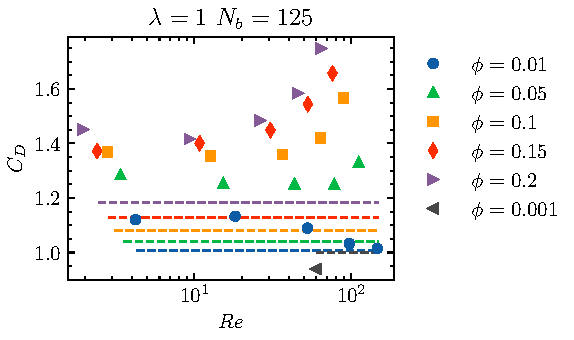
\includegraphics[height = 0.35\textwidth]{image/HOMOGENEOUS/fCA/Cp_N_5_l_1.pdf}
    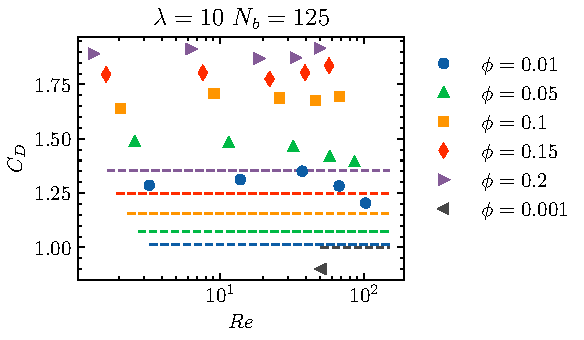
\includegraphics[height = 0.35\textwidth]{image/HOMOGENEOUS/fCA/Cp_N_5_l_10.pdf}
    
    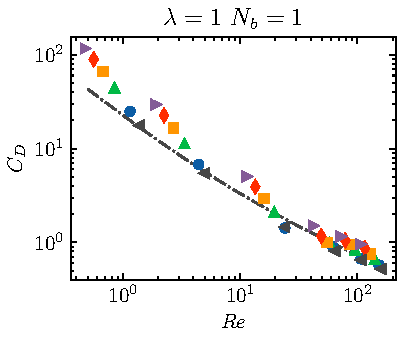
\includegraphics[height = 0.35\textwidth]{image/HOMOGENEOUS/fCA/Cp_N_1_l_1.pdf}
    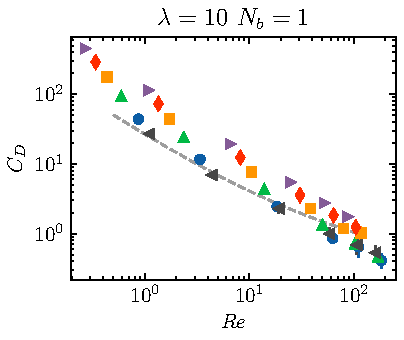
\includegraphics[height = 0.35\textwidth]{image/HOMOGENEOUS/fCA/Cp_N_1_l_10.pdf}

    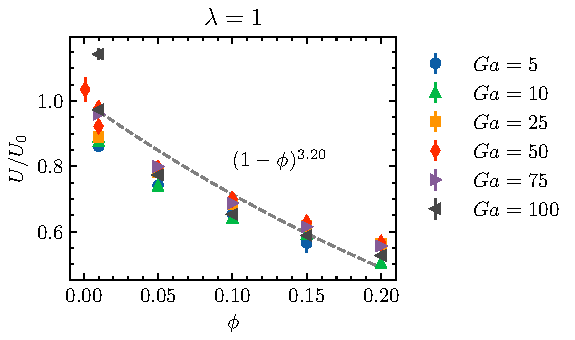
\includegraphics[height = 0.35\textwidth]{image/HOMOGENEOUS/fCA/Re_iso_N_5_l_1.pdf}
    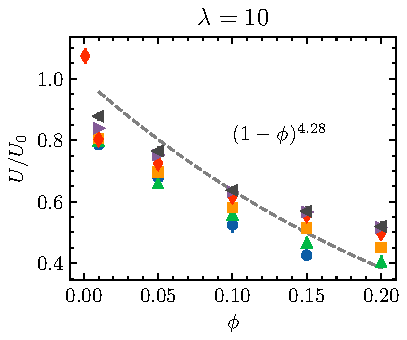
\includegraphics[height = 0.35\textwidth]{image/HOMOGENEOUS/fCA/Re_iso_N_5_l_10.pdf}
    \caption{
        Drag coef(top)ficient and dimensionless force for ordered $N_b=1$ array and unordered arrays $N_b=125$. 
        The symbols correspond to different volume fraction ($\blacktriangleleft$) $\phi = 0.1$\%, ($\bullet$) $\phi = 1\%$, ($\blacktriangle$) $\phi = 5\%$, ($\blacksquare$) $\phi = 10\%$, ($\blacklozenge$) $\phi = 15\%$, and ($\blacktriangleright$) $\phi = 20$\%.
        (bottom) Reynolds number $Re^* = Re / Re_\text{Magnaudet}$ where $Re$ is the Reynolds number based on the drift velocity of the DNS and $Re_\text{Magnaudet}$ is the Reynolds number as a function of $Ga$ predicted by \citet{magnaudet1997forces} formula (6).  
        The symbols correspond to different volume fraction ($\bullet$) $\phi = 1\%$, ($\blacktriangle$) $\phi = 5\%$, ($\blacksquare$) $\phi = 10\%$, ($\blacklozenge$) $\phi = 15\%$ and ($\blacktriangleright$) $\phi = 20\%$.
    }
    \label{fig:Cp}
\end{figure}

\begin{figure}[h!]
    \centering    
    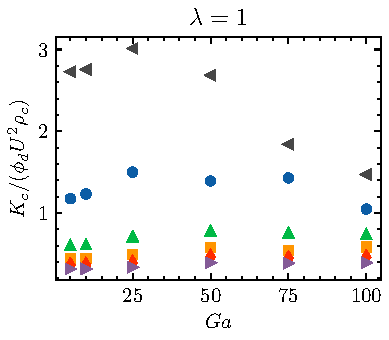
\includegraphics[height = 0.35\textwidth]{image/HOMOGENEOUS/fCA/Tf_N_1_l_1.pdf}
    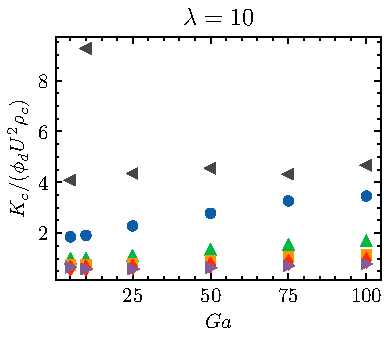
\includegraphics[height = 0.35\textwidth]{image/HOMOGENEOUS/fCA/Tf_N_1_l_10.pdf}

    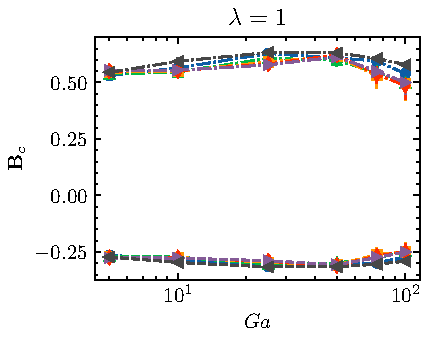
\includegraphics[height = 0.35\textwidth]{image/HOMOGENEOUS/fCA/Bf_N_1_l_1.pdf}
    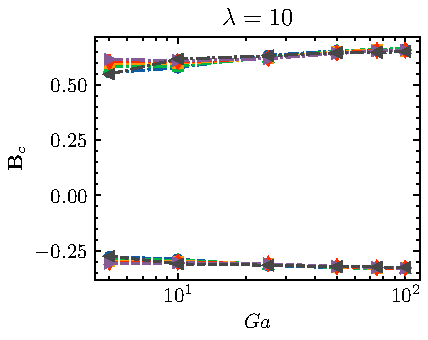
\includegraphics[height = 0.35\textwidth]{image/HOMOGENEOUS/fCA/Bf_N_1_l_10.pdf}
   \caption{
        (top) dimensionless fluid pseudo turbulent energy. 
        (bottom) deviatoric components of the matic B
        The symbols correspond to different volume fraction ($\blacktriangleleft$) $\phi = 0.1$\%, ($\bullet$) $\phi = 1\%$, ($\blacktriangle$) $\phi = 5\%$, ($\blacksquare$) $\phi = 10\%$, ($\blacklozenge$) $\phi = 15\%$, and ($\blacktriangleright$) $\phi = 20$\%.
    }
    \label{fig:Cp}
\end{figure}


On \ref{fig:Cp}(bottom) we can see that the formula of Rvikind and Ryskin (1976) is valid only in the low inertial regime which is probably due to the wake of the particles in tri periodic domain.